\documentclass[hyperref={bookmarksopen=false}]{beamer} 

\usepackage[english]{babel}
\usepackage{pgf,pgfarrows,pgfnodes,pgfautomata,pgfheaps,pgfshade}
\usepackage{ngerman}
\usepackage[latin1]{inputenc}

\usepackage{graphicx}

\useoutertheme[section]{tubs}

%\setbeamertemplate{itemize items}[ball]
%\setbeamertemplate{itemize items}[square]
\setbeamertemplate{itemize items}[tusquare]

\subtitle{Labor Android Programmierung - Final presentation}
\title{LDAP Contact Sync} 
\author[C. Gerloff und T. Lorentzen]{Till Lorentzen und Christopher Gerloff}
\institute[TU Braunschweig, IBR]{Technische Universit�t Braunschweig, IBR}

\date{\today}

\instlogo{ibr_deu}
%\titlegraphic{iz}
\titlegraphic{iz_corner}



\begin{document}

\frame[plain]{\titlepage} 

\setbeamercolor{frametitle}{fg=white,bg=tu-red}
\frame{
        \frametitle{Einleitung}
        \tableofcontents
        }
\setbeamercolor{frametitle}{fg=black,bg=tu-grey}


\section{Projektziel}

\frame{
 \frametitle{Motivation \& Ziel} 
 \begin{block}{Motivation}
 \begin{itemize}
    \item Kontaktsynchronisation mit vorhandenen Kontaktdatenbanken sehr wichtig
    \item LDAP Verzeichnisse sehr verbreitet
    \item Von Haus aus keine M�glichkeit auf LDAP Verzeichnisse zuzugreifen

 \end{itemize}
 \end{block}
  \begin{block}{Ziel}
 \begin{itemize}
    \item Integration in das interne Kontaktbuch und Synchronisation von Kontakten aus LDAP Verzeichnissen

 \end{itemize}
 \end{block}
 
}

\section{Anforderungen}

\frame{
 \frametitle{Synchronisation mit LDAP Kontakten} 
 \begin{block}{Funktionale Anforderungen}
 \begin{itemize}
    \item Verbindung zu LDAP Server herstellen
    \item Kontakte des LDAP Servers durchsuchen
    \item Kontakte in das Kontaktbuch des Mobiltelefons importieren
    \item Importierte Kontakte ggf. mit vorhandenen Kontakten zusammenf�hren
    \item Bei �nderungen eines Kontakts, Server und Telefon synchronisieren

 \end{itemize}
 \end{block}
 
 \
}

\frame{
 \frametitle{Synchronisation mit LDAP Kontakten} 
 \begin{block}{Nicht-funktionale Anforderungen}
 \begin{itemize}
    \item Intuitive Bedienung
    \item So wenig GUI wie m�glich
    \item Hohe Integration in die vorhandenen Systemstrukturen
    \item Geringe Akkubelastung

 \end{itemize}
 \end{block}
}

\section{Projektplan}

\frame{
\frametitle{Projektplan}
  \begin{block}{Zeitplan}
    \center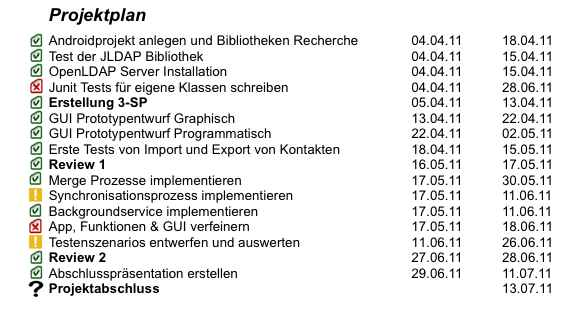
\includegraphics[width=0.9\textwidth]{projektplan.png}\\
  \end{block}
}

\section{Grundlagen}
\frame{
 \frametitle{Wichtige Komponenten} 
\begin{block}{AccountManager}
 \begin{itemize}
   \item Speichert alle LDAP Accounts, mit denen synchronisiert werden soll
   \item Android �bernimmt die Speicherung
 \end{itemize}
 \end{block}
    \begin{block}{AccountAuthenticator}
    \begin{itemize}
      \item Schnittstelle um einen Account hinzuzuf�gen 
      \item Ruft die AddServer Activity aus den Einstellungen auf
      \item Speichert die Eingaben als Account ab
    \end{itemize}
 \end{block}
}

\frame{
 \frametitle{Wichtige Komponenten} 
 \begin{block}{RawContacts}
    \begin{itemize}
        \item Kontaktdaten werden pro Account gespeichert
	\item Sichtbarkeit im Kontaktbuch je nach Wunsch 
    \end{itemize}
 \end{block}
\begin{block}{ContactManager}
 \begin{itemize}
   \item ...
   \item ...
 \end{itemize}
 \end{block}
 \begin{block}{ContactUtils}
 \begin{itemize}
   \item ...
   \item ...
 \end{itemize}
 \end{block}
}

\frame{
\frametitle{Contact Database}
  \begin{block}{Datenstruktur der Kontakte}
    \center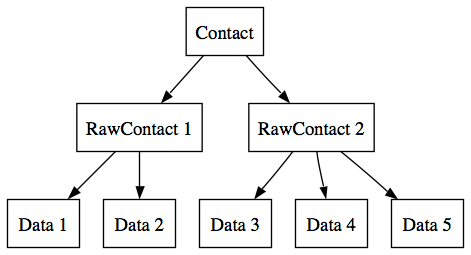
\includegraphics[width=0.8\textwidth]{contacts-2.png}\\
    \tiny{Quelle: http://developer.android.com/resources/articles/contacts.html}
  \end{block}
}

\frame{
 \frametitle{Wichtige Komponenten} 

 \begin{block}{SyncAdapter}
    \begin{itemize}
        \item Schnittstelle f�r Android zur Synchronisation
    \end{itemize}
 \end{block}

   \begin{block}{LDAPSyncService}
    \begin{itemize}
        \item Ersetz den ContentProvider
    \end{itemize}
 \end{block}
}


\section{Probleme}

\frame{
 \frametitle{Synchronisation mit LDAP Kontakten} 
 \begin{block}{Potenzielle Hindernisse}
 \begin{itemize}
    \item Integrationsprobleme in die Standard Kontakte des Android Betriebssystems
    \begin{itemize}
    \item Integration eigener Views in die App
 \end{itemize}
    \item Stromverbrauch zu hoch
    \begin{itemize}
    \item Anpassung des Synchronisationsverhaltens an die Akkuleistung
 \end{itemize}
    \item Aenderungen im LDAP Verzeichnis k�nnen nicht erkannt werden
    \begin{itemize}
    \item Push Server (nicht Teil dieses Projektes)
 \end{itemize}
    \item Inkompatibilit�t der OpenLDAP Bibliothek
    \begin{itemize}
    \item Recherche und Verwendung anderer Bibliotheken
 \end{itemize}

 \end{itemize}
 \end{block}
}

\frame{
	\frametitle{Tats�chliche Probleme}
	
 	  \begin{block}{Tats�chliche Probleme}
   	      \begin{itemize}
                  \item OpenLDAP Bibliothek veraltet
                  \item Nahtlose Integration in die vorhandene Kontakte Anwendung nicht m�glich
		  \item Probleme beim Mapping zwischen statischen und dynamischen Feldern
		  \item ...
		  \item ...
                  \item ...
                  \item ...
                \end{itemize}
           \end{block}
}

\frame{
	\frametitle{L�sungen}
	
 	  \begin{block}{L�sungen}
   	      \begin{itemize}
	      \item Einsatz des LDAP SDK von UnboundID
                  \item Eigener Kontakteditor
                    \begin{itemize}
                      \item Aufgerufen durch Intent aus der Kontakte Anwendung
                    \end{itemize}
                  
		  \item Umsetzung als Service
		  \item ...
		  \item ...
                  \item ...
                  \item ...
                \end{itemize}
           \end{block}
}

\frame{
	\frametitle{Demo}
	\begin{block}{}
	\center \bf{\LARGE{DEMO}}
	\end{block}
}

\frame{
  \frametitle{Teamwork}
  \begin{block}{Git \& GitHub}
    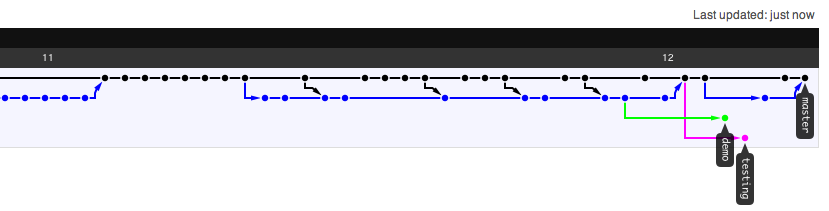
\includegraphics[scale=0.35]{git.png}\\
    \tiny{ https://www.github.com/soneyworld/AndroidLab}\\
    \tiny{\$ git clone git://github.com/soneyworld/AndroidLab.git AndroidLab}
  \end{block}
  }

\frame{
  \frametitle{Projektstatus}
   \begin{block}{Projektstatus}
   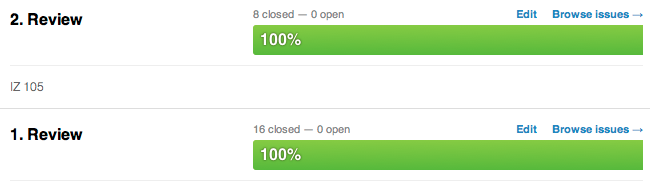
\includegraphics[scale=0.4]{status2.png}
   \end{block}
   \begin{block}{}
    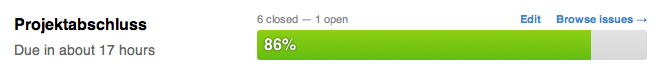
\includegraphics[scale=0.4]{status.png}\\
    \tiny{ https://github.com/soneyworld/AndroidLab/issues/milestones}
  \end{block}
}



\section{Ausblick}

\frame{
 \frametitle{Ausblick} 
 \begin{block}{In Zukunft}
 \begin{itemize}
    \item Funktionalit�t und Design verbessern
    \item Lizenz? Ver�ffentlichung?
 \end{itemize}
 \end{block}
}

\frame{
  \frametitle{Fragen?}
  \begin{block}{Antworten!}
   
  \end{block}

  \begin{block}{Weitere Informationsquellen}
  \begin{itemize}
    \item Wiki: \tiny{https://github.com/soneyworld/AndroidLab/wiki}\normalsize
    \item Twitter: \tiny{https://twitter.com/ldapsync}
  \end{itemize}
  \end{block}
}

\end{document}   
